%
% $RCSfile: structure.tex,v $
%
% Copyright (C) 2002-2008. Christian Heller.
%
% Permission is granted to copy, distribute and/or modify this document
% under the terms of the GNU Free Documentation License, Version 1.1 or
% any later version published by the Free Software Foundation; with no
% Invariant Sections, with no Front-Cover Texts and with no Back-Cover
% Texts. A copy of the license is included in the section entitled
% "GNU Free Documentation License".
%
% http://www.cybop.net
% - Cybernetics Oriented Programming -
%
% http://www.resmedicinae.org
% - Information in Medicine -
%
% Version: $Revision: 1.1 $ $Date: 2008-08-19 20:41:09 $ $Author: christian $
% Authors: Christian Heller <christian.heller@tuxtax.de>
%

\section{Structure}
\label{structure_heading}
\index{Structure of this Book}

This document is divided into fourteen chapters. Neglecting this introduction,
thirteen chapters remain which are organised in four parts. They are illustrated
in figure \ref{structure_figure}.

\begin{figure}[ht]
    \begin{center}
        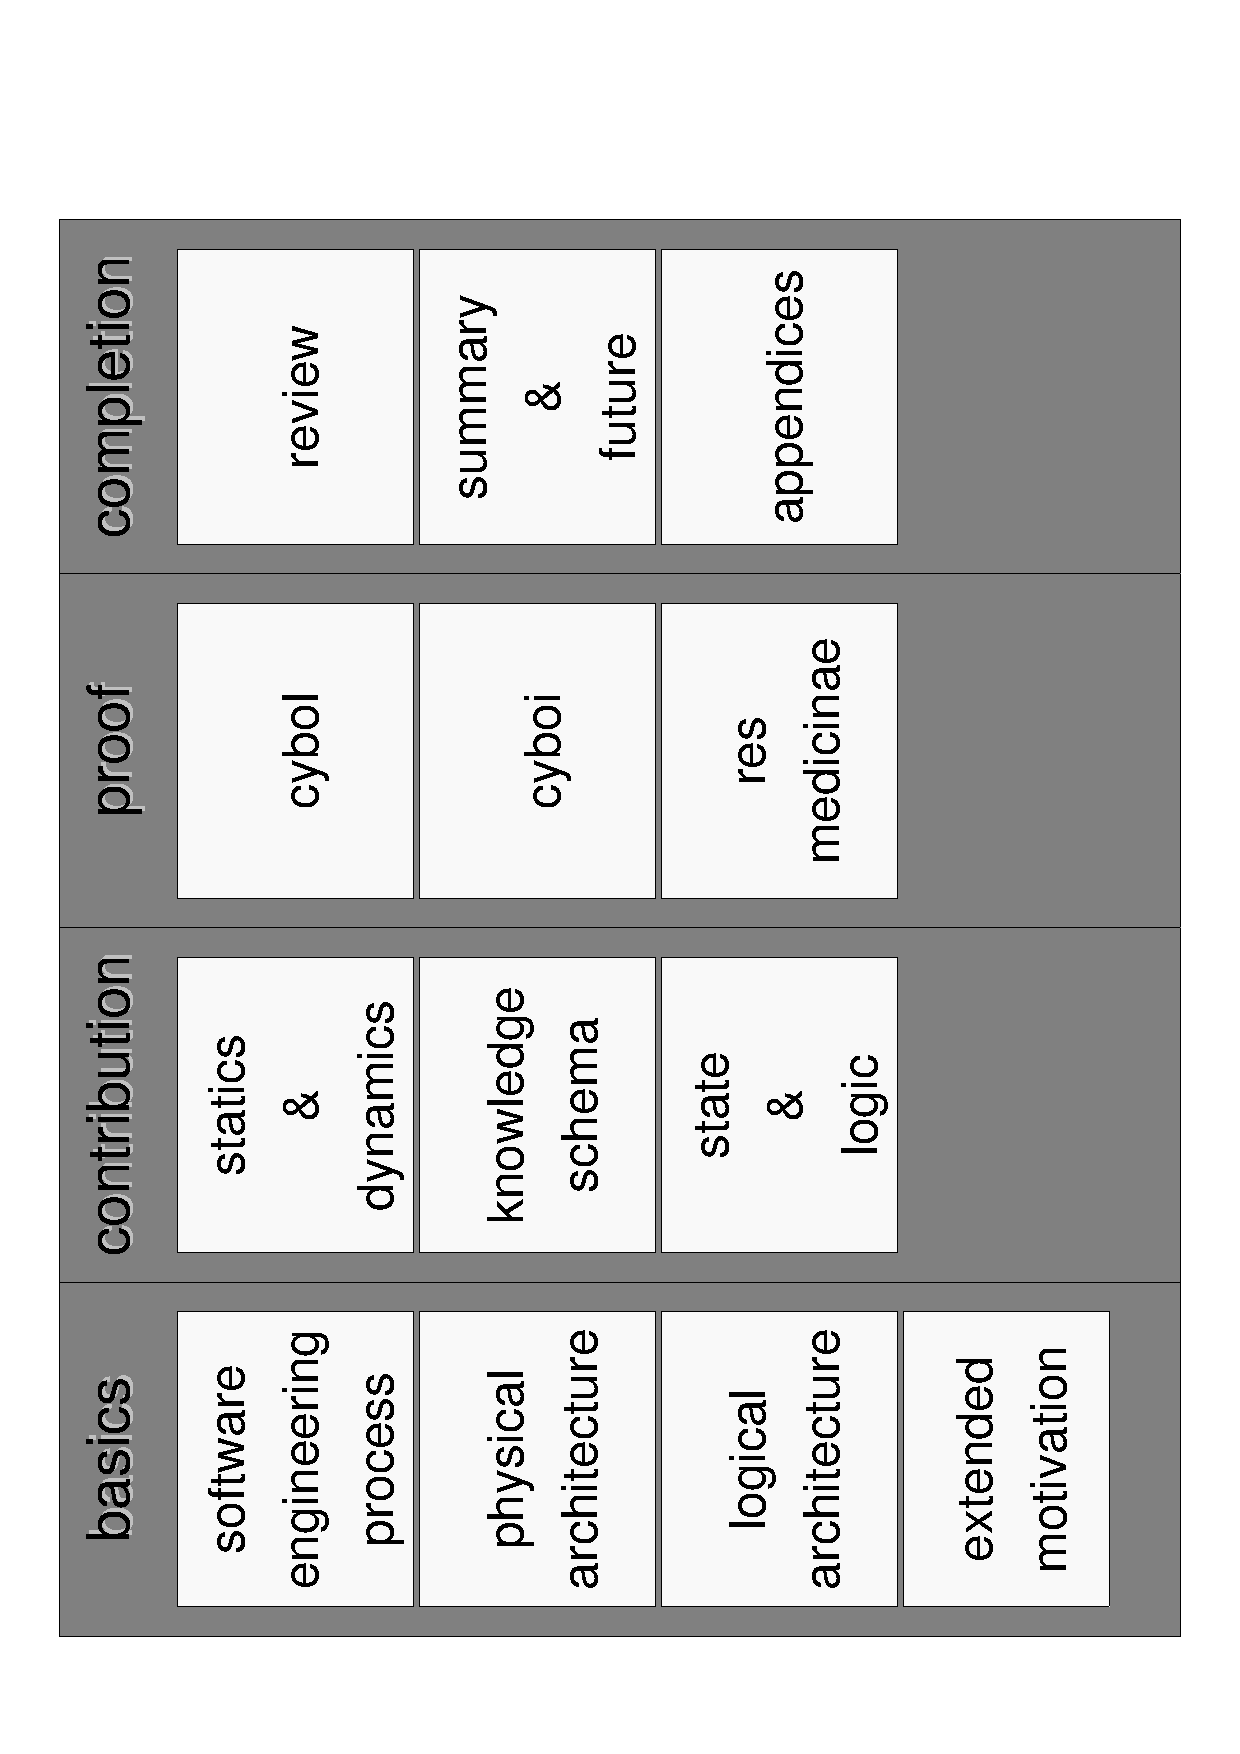
\includegraphics[scale=0.3,angle=-90]{graphic/structure.pdf}
        \caption{Document Structure}
        \label{structure_figure}
    \end{center}
\end{figure}

Part \ref{basics_heading} considers basic concepts of software development
(\emph{State of the Art}), before the then following part \ref{contribution_heading}
contributes new concept ideas. Practical proof of their operability is given in
part \ref{proof_heading}. And part \ref{completion_heading} finally completes
the work with a review, summary and outlook into the future.

\emph{Software Engineering Processes} (SEP) (chapter
\ref{software_engineering_process_heading}) have to be briefly described to be
able to estimate the effects of abstraction changes on the actual SEP phases.
The \emph{Physical Architecture} (chapter \ref{physical_architecture_heading})
of a standard \emph{Information Technology} (IT) environment is necessary
background knowledge for later reflections on the design of software systems
and their communication paradigms. Finally, the \emph{Logical Architecture}
(chapter \ref{logical_architecture_heading}), that is conceptual solutions for
structuring software systems, is investigated, to later be able to possibly
find \emph{Pros} and \emph{Cons}.

A short \emph{Recapitulation} of introduced state-of-the-art concepts and the
idea of an \emph{inter-disciplinary}, \emph{cybernetics-oriented} approach lead
to an \emph{Extended Motivation} (chapter \ref{extended_motivation_heading})
whose results and solutions are described in the remaining parts of the work.

A first description focuses on the distinction of \emph{Statics and Dynamics}
(chapter \ref{statics_and_dynamics_heading}). In a second step, a new kind of
\emph{Knowledge Schema} gets introduced (chapter \ref{knowledge_schema_heading}).
Thirdly, \emph{State and Logic} are described as to-be-separated knowledge
models (chapter \ref{state_and_logic_heading}).

The application of the merged traditional and new design concepts results in
the XML-based \emph{Cybernetics Oriented Language} (CYBOL) (chapter
\ref{cybernetics_oriented_language_heading}). A corresponding
\emph{Cybernetics Oriented Interpreter} (CYBOI) (chapter
\ref{cybernetics_oriented_interpreter_heading}) is needed to execute systems
defined in that language. The \emph{Res Medicinae} prototype application
(chapter \ref{res_medicinae_heading}) is written in CYBOL and executed by
CYBOI.

One might argue that chapters \ref{cybernetics_oriented_language_heading}
(CYBOL) and \ref{cybernetics_oriented_interpreter_heading} (CYBOI) should
rather belong to part \ref{contribution_heading}, called \emph{Contribution},
since they contain newly developed technologies. However, as they were needed
for the practical proof, and in order to keep the chapter symmetry, they were
placed in part \ref{proof_heading}, called \emph{Proof}.

After a \emph{Review} validating and evaluating the CYBOP programming philosophy
in comparison to the original motivation (chapter \ref{review_heading}), a
\emph{Summary} and recommendations for \emph{Future} research are given
(chapter \ref{summary_and_outlook_heading}). The \emph{Appendices} (chapter
\ref{appendices_heading}) contain used abbreviations, references to literature
and the usual lists of figures and tables. A glossary was omitted since this
document does not want to be a lexicon. All terms are explained at their first
appearance in the text. A short history of thoughts that lead to the creation
of this document and recommendations for a migration to CYBOL as well as some
licences in full text follow. Caution! The page numbers behind an index entry
at the end of this document refer to the \emph{Beginning} of the section in
which the entry appeared.
